%-----------------------------------------------------------------------------%
\chapter{\babSatu}
%-----------------------------------------------------------------------------%
% \todo{tambahkan kata-kata pengantar bab 1 disini}


% %-----------------------------------------------------------------------------%
% \section{Latar Belakang}
% %-----------------------------------------------------------------------------%
% \todo{tuliskan latar belakang penelitian disini}


% %-----------------------------------------------------------------------------%
% \section{Permasalahan}
% %-----------------------------------------------------------------------------%
% Pada bagian ini akan dijelaskan mengenai definisi permasalahan 
% yang \saya~hadapi dan ingin diselesaikan serta asumsi dan batasan 
% yang digunakan dalam menyelesaikannya.


% %-----------------------------------------------------------------------------%
% \subsection{Definisi Permasalahan}
% %-----------------------------------------------------------------------------%
% \todo{Tuliskan permasalahan yang ingin diselesaikan. Bisa juga
% 	berbentuk pertanyaan}


% %-----------------------------------------------------------------------------%
% \subsection{Batasan Permasalahan}
% %-----------------------------------------------------------------------------%
% \todo{Umumnya ada asumsi atau batasan yang digunakan untuk 
% 	menjawab pertanyaan-pertanyaan penelitian diatas.}


% %-----------------------------------------------------------------------------%
% \section{Tujuan}
% %-----------------------------------------------------------------------------%
% \todo{Tuliskan tujuan penelitian.}


% %-----------------------------------------------------------------------------%
% \section{Posisi Penelitian}
% %-----------------------------------------------------------------------------%
% \todo{Posisi penelitian Anda jika dilihat secara bersamaan dengan 
% 	peneliti-peneliti lainnya. Akan lebih baik lagi jika ikut menyertakan 
% 	diagram yang menjelaskan hubungan dan keterkaitan antar 
% 	penelitian-penelitian sebelumnya}


% %-----------------------------------------------------------------------------%
% \section{Metodologi Penelitian}
% %-----------------------------------------------------------------------------%
% \todo{Tuliskan metodologi penelitian yang digunakan.}


% %-----------------------------------------------------------------------------%
% \section{Sistematika Penulisan}
% %-----------------------------------------------------------------------------%
% Sistematika penulisan laporan adalah sebagai berikut:
% \begin{itemize}
% 	\item Bab 1 \babSatu \\
% 	\item Bab 2 \babDua \\
% 	\item Bab 3 \babTiga \\
% 	\item Bab 4 \babEmpat \\
% 	\item Bab 5 \babLima \\
% 	\item Bab 6 \babEnam \\
% 	\item Bab 7 \kesimpulan \\
% \end{itemize}

% \todo{Tambahkan penjelasan singkat mengenai isi masing-masing bab.}

\section{Project Sponsor}

\begin{table}[h!]
    \centering
    \begin{tabular}{|l|l|}
        \hline
        \textbf{Nama} & Haykal Rasidi \\ \hline
        \textbf{Jabatan} & IT Infrastruktur Manager \\ \hline
        \textbf{Kontak} & +62 813-8044-7624 \\ \hline
    \end{tabular}
\end{table}

\section{Business Needs}

Issue ini berawal dari keresahan beberapa karyawan network engineer di tempat saya bekerja dalam melakukan konfigurasi perintah/command yang berulang ke banyak perangkat. Untuk melakukan hal tersebut memerlukan beberapa engineer yang tujuannya agar pekerjaan yang dilakukan lebih cepat selesai. 

Permasalahan berikutnya jika perangkat yang akan dikonfigurasi semakin hari semakin bertambah dan konfigurasi perintah/command semakin panjang, maka engineer dan waktu yang dibutuhkan untuk menyelesaikan proses tersebut juga semakin bertambah.  

Permasalahan lain, faktor human error akan semakin besar dalam melakukan konfigurasi yang berulang dan ke banyak perangkat. 

Oleh karena itu perlu adanya system yang mampu menyederhanakan proses tersebut agar menjadi efektif dan lebih efisien. 

\begin{tabular}{|>{\raggedright\arraybackslash}p{4cm}|>{\raggedright\arraybackslash}p{4cm}|>{\raggedright\arraybackslash}p{3.5cm}|}
\hline
\textbf{Harapan} & \textbf{Kenyataan} & \textbf{Masalah} \\
\hline
Tidak memerlukan sumber daya manusia yang terlalu banyak dalam melakukan konfigurasi ke banyak perangkat. & Saat ini dalam melakukan konfigurasi ke banyak perangkat diperlukan beberapa sumber daya manusia. & Diperlukan suatu sistem informasi yang mampu mengintegrasikan seluruh perangkat dalam satu dashboard dalam melakukan konfigurasi perintah/command secara bersamaan dalam satu waktu. \\
\hline
Tidak memerlukan waktu yang terlalu lama dalam melakukan banyak proses ke banyak perangkat. & Saat ini waktu yang dibutuhkan akan bertambah jika perangkat dan konfigurasi yang dilakukan semakin banyak. & \\
\hline
Mengurangi human error dalam melakukan konfigurasi yang panjang ke banyak perangkat dalam waktu yang singkat. & Sering terjadi kesalahan dalam melakukan konfigurasi perintah/command atau ada step yang terlewat. & \\
\hline
Sistem yang mengintegrasikan banyak perangkat dalam satu dashboard untuk memudahkan dalam manajemen konfigurasi. & Belum ada sistem yang mengintegrasikan, saat ini dalam melakukan konfigurasi dilakukan satu persatu dengan membuka akses terhadap tiap perangkat. & \\
\hline
\end{tabular}


% insert gambar network automation

\begin{figure}
	\centering
	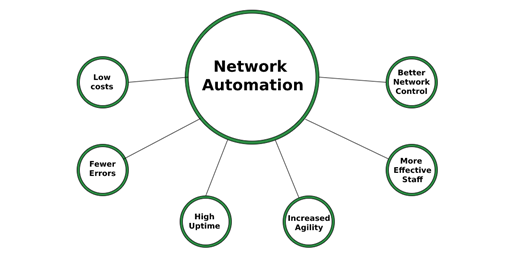
\includegraphics[width=0.70\textwidth]
		{assets/pics/Network Automation.png}
	\caption{Network Automation}
	\label{fig:NetworkAutomation}
\end{figure}


Network Automation menjadi sebuah solusi atas beberapa permasalahan tersebut, mulai dari biaya yang tinggi untuk hire beberapa sumber daya untuk melakukan pekerjaan tersebut, menyederhanakan sebuah proses yang kompleks dan panjang hingga menghindari banyaknya kesalahan dalam melakukan konfigurasi. Network automation sebuah solusi yang diimplementasikan dalam bentuk sistem yang akan menunjang suatu proses bisnis perusahaan dari sisi IT infrastruktur.

\subsection{Non-Functional Requirements (NFR)}
\begin{enumerate}
    \item \textbf{Scalability (Skalabilitas)}: Kemampuan sistem untuk menangani peningkatan jumlah perangkat jaringan.
    
    \item \textbf{Performance (Kinerja)}
    \begin{itemize}
        \item Latency rendah dalam pengiriman konfigurasi atau perubahan jaringan.
        \item Sistem otomatisasi harus dapat menangani volume besar tugas-tugas konfigurasi secara bersamaan.
    \end{itemize}
    
    \item \textbf{Security (Keamanan)}
    \begin{itemize}
        \item Proses otomatisasi harus mematuhi standar keamanan yang tinggi untuk mencegah akses tidak sah atau modifikasi pada konfigurasi jaringan.
        \item Enkripsi data: Semua data yang dikirimkan melalui jaringan dan proses otomatisasi harus terenkripsi.
        \item Authentication \& Authorization: Sistem harus memastikan hanya pengguna yang sah dapat menjalankan tugas otomatisasi dan harus ada kontrol akses yang ketat.
    \end{itemize}
    
    \item \textbf{Usability (Kemudahan Penggunaan)}
    \begin{itemize}
        \item Dashboard otomatisasi jaringan harus intuitif dan mudah digunakan oleh admin jaringan tanpa membutuhkan pelatihan yang terlalu intensif.
        \item Error handling yang jelas: Pesan kesalahan dan status operasional harus mudah dipahami oleh pengguna.
    \end{itemize}
    
    \item \textbf{Interoperability (Interoperabilitas)}
    \begin{itemize}
        \item Sistem otomatisasi harus dapat berfungsi dengan baik di berbagai perangkat dan vendor jaringan yang berbeda.
        \item Standar terbuka: Memastikan kompatibilitas dengan berbagai protokol jaringan dan perangkat keras yang digunakan.
    \end{itemize}
    
    \item \textbf{Availability (Ketersediaan)}
    \begin{itemize}
        \item Sistem otomatisasi harus selalu tersedia untuk digunakan kapan saja.
        \item High availability (Ketersediaan tinggi): Sistem harus memiliki redundansi untuk menghindari downtime.
    \end{itemize}
    
    \item \textbf{Auditability (Kemampuan Audit)}: Sistem harus mendukung kemampuan untuk melacak semua perubahan konfigurasi jaringan dan menyediakan log atau laporan audit yang komprehensif.
    
    \item \textbf{Flexibility (Fleksibilitas)}: Kemampuan sistem untuk beradaptasi dengan kebutuhan yang terus berubah dan berkembang, termasuk mendukung teknologi baru atau perubahan dalam arsitektur jaringan.
\end{enumerate}

Secara umum, fungsi non-fungsional dalam network automation menekankan aspek kualitas sistem yang berkaitan dengan bagaimana sistem beroperasi, bukan hanya apa yang dapat dilakukan oleh sistem tersebut.

\subsection{Functional Requirements}
\begin{enumerate}
    \item \textbf{Pengelolaan Konfigurasi (Configuration Management)}
    \begin{itemize}
        \item Membuat, menyimpan, dan menerapkan perubahan konfigurasi perangkat jaringan secara otomatis.
        \item Melakukan backup dan restore konfigurasi perangkat jaringan.
    \end{itemize}
    
    \item \textbf{Orkestrasi Jaringan}
    \begin{itemize}
        \item Mengkoordinasikan beberapa proses otomatisasi sekaligus di berbagai perangkat atau segmen jaringan.
        \item Integrasi dengan berbagai platform atau perangkat lunak jaringan yang berbeda, sehingga seluruh infrastruktur jaringan dapat diatur secara konsisten.
    \end{itemize}
    
    \item \textbf{Integrasi dengan Sistem Manajemen Jaringan Lain}
    \begin{itemize}
        \item Berfungsi sebagai penghubung dengan alat manajemen jaringan lainnya seperti SDN (Software Defined Networking), NFV (Network Functions Virtualization), dan platform monitoring untuk orkestrasi yang lebih luas.
    \end{itemize}
\end{enumerate}

Fungsi-fungsi tersebut berfokus pada bagaimana otomatisasi jaringan dapat membantu administrator jaringan mengelola infrastruktur secara efisien, mengurangi kesalahan manual, meningkatkan kecepatan, serta memastikan stabilitas dan keamanan.

\section{Business Value}

\subsection{Tangible Business Value (Nilai Bisnis yang Terukur/Terlihat)}
\begin{itemize}
    \item \textbf{Pengurangan Biaya Operasional}: Otomasi jaringan mengurangi kebutuhan akan intervensi manual, sehingga menghemat biaya tenaga kerja dan mempercepat penyelesaian tugas operasional.
    \item \textbf{Efisiensi Jaringan}: Dengan proses otomatisasi, jaringan dapat dioptimalkan secara efisien, sehingga meningkatkan pemanfaatan sumber daya jaringan dan mengurangi biaya infrastruktur.
    \item \textbf{Pengurangan Waktu Downtime}: Network automation memungkinkan deteksi dan perbaikan masalah lebih cepat, yang berarti waktu downtime jaringan berkurang, meningkatkan produktivitas.
    \item \textbf{Peningkatan Skala (Scalability)}: Otomasi memungkinkan perusahaan mengelola jaringan yang lebih besar tanpa perlu menambah jumlah personel teknis, sehingga memberikan skala yang lebih baik untuk ekspansi bisnis.
    \item \textbf{Kecepatan Implementasi}: Penerapan layanan dan konfigurasi jaringan menjadi lebih cepat dan akurat, yang memungkinkan perusahaan merespons kebutuhan bisnis dengan lebih cepat.
\end{itemize}

\subsection{Intangible Business Value (Nilai Bisnis yang Tidak Terlihat/Tidak Terukur Langsung)}
\begin{itemize}
    \item \textbf{Peningkatan Kualitas Layanan}: Dengan otomatisasi, perusahaan dapat memberikan layanan yang lebih stabil, minim gangguan, dan lebih responsif terhadap kebutuhan pelanggan.
    \item \textbf{Inovasi Lebih Cepat}: Otomasi jaringan membebaskan waktu dan sumber daya tim TI untuk fokus pada inovasi dan peningkatan layanan daripada tugas-tugas rutin.
    \item \textbf{Peningkatan Kepuasan}: Ketersediaan jaringan yang lebih baik dan peningkatan responsivitas layanan meningkatkan pengalaman pengguna, yang berkontribusi pada kepuasan pelanggan.
    \item \textbf{Ketahanan (Resilience)}: Otomasi membantu membangun jaringan yang lebih tangguh terhadap perubahan dan kegagalan, sehingga bisnis dapat terus berjalan dengan gangguan minimal.
\end{itemize}

\section{Special Issues}
\begin{enumerate}
    \item \textbf{Kompleksitas Infrastruktur yang Beragam}: Jaringan modern sering kali terdiri dari berbagai perangkat keras, vendor, dan teknologi yang berbeda (misalnya router, switch, firewall dari berbagai merek). Masing-masing perangkat mungkin memiliki protokol dan API yang berbeda untuk diotomatisasi, sehingga menyulitkan pengelolaan dengan satu solusi universal.
    
    \item \textbf{Keamanan (Security)}: Otomatisasi jaringan dapat meningkatkan risiko jika tidak dikelola dengan baik. Skrip otomatisasi yang salah atau memiliki kerentanan dapat membuka celah bagi penyerang.
    
    \item \textbf{Skalabilitas}: Ketika jaringan tumbuh besar dan kompleks, alat otomasi harus mampu menyesuaikan dan berfungsi dengan baik di lingkungan besar. Masalah skalabilitas ini dapat mencakup performa alat otomasi, manajemen database, atau integrasi dengan sistem lain.
    
    \item \textbf{Pengelolaan Perubahan (Change Management)}: Proses otomatisasi dapat menyebabkan perubahan di jaringan dengan cepat dan dalam skala besar. Jika tidak dikelola dengan baik, perubahan yang tidak diverifikasi bisa merusak konfigurasi dan menyebabkan downtime.
    
    \item \textbf{Kurangnya Standardisasi}: Tidak semua vendor atau organisasi menggunakan standar yang sama dalam mengimplementasikan jaringan. Hal ini menciptakan tantangan dalam mengintegrasikan alat otomatisasi.
    
    \item \textbf{Kebutuhan Skill yang Khusus}: Mengimplementasikan otomatisasi jaringan memerlukan keterampilan baru bagi tim jaringan, seperti pemrograman, pemahaman API, dan penguasaan alat otomasi. Tim jaringan tradisional mungkin perlu waktu untuk menyesuaikan diri dengan teknologi baru ini.
    
    \item \textbf{Kendala Kompatibilitas dengan Teknologi Lama (Legacy Systems)}: Banyak jaringan masih menggunakan perangkat atau sistem lama yang tidak mendukung otomatisasi modern, sehingga sulit untuk mengintegrasikannya ke dalam proses otomatisasi.
\end{enumerate}



